\chapter{Estado del arte}

Actualmente, el estado del mercado para este tipo de desarrollos está muy limitado dado que 
la mayoría de los datos que se tratan son de carácter sensible. Por tanto, se 
debe tener un especial cuidado con el tratamiento de los mismos tanto a la hora de transmitirlos
como en su almacenamiento. Además, al ser una aplicación que será utilizada en organismos públicos 
tiene que pasar por un largo proceso burocrático ya que las acciones que se pueden realizar con este
tipo de sistemas son muy delicadas. Cualquier fallo puede causar un gran problema a uno o varios ciudadanos.\\

Por tanto, las aplicaciones orientadas a solucionar este problema son una gran minoría. En este apartado nos vamos a centrar en los dos más conocidas dentro del sector.

\section{GESPOL GPSS PDA}
La primera de las aplicaciones que encontramos es \textbf{GESPOL GPSS PDA}\cite{gespol} creada por \textit{GESPOL}. Su especialidad es el desarrollo de 
aplicaciones dedicadas específicamente a la Administración Pública.\\

Esta aplicación realiza un gran número de actividades entre ellas:

\begin{itemize}
	\item Control de acceso a usuarios.
	\item Posicionamiento GPS del agente.
	\item Gestión de incidencias.
	\item Gestión de anomalías en la vía pública.
	\item Gestión de denuncias de tráfico.
	\item Consulta a la DGT.
	\item Impresión de multas.
\end{itemize}

Este es el aspecto que tiene la aplicación: 

\begin{figure}[H]
	\centering
	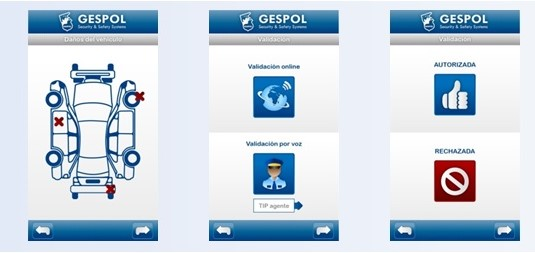
\includegraphics[scale=0.75]{imagenes/gespol2.jpg}
	\caption{Validación de usuario y daños de vehículos en GESPOL.\cite{gespol} \label{fig:figura16}}
\end{figure}

\begin{figure}[H]
	\centering
	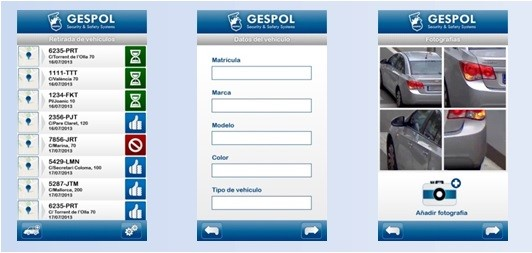
\includegraphics[scale=0.75]{imagenes/gespol1.jpg}
	\caption{Retirada, daños y fotografías de vehículos en GESPOL.\cite{gespol} \label{fig:figura17}}
\end{figure}

El principal problema de esta aplicación es que está bastante desactualizada. El desarrollo se terminó y no se han incluido mejoras en el software. Además,
es una aplicación de pago y no es de código libre, por lo que no la podemos utilizar para continuar su desarrollo con nuevas funcionalidades y adaptada a las tecnologías recientes.

\section{Appolo}
La segunda aplicación a analizar se llama \textbf{Appolo} y ha sido creada por la empresa \textit{Almerimatik Sistemas Informáticos S.A}. \\

\textit{Appolo} es un sistema informático para la gestión completa de los Cuerpos de Policía Local y afirman que es un sistema
flexible, abierto y que están en permanente evolución debido a las necesidades de sus usuarios.\\

Algunas de las funcionalidades que ofrece son las siguientes:
\begin{itemize}
	\item Gestiona el seguimiento de la actividad de los agentes.
	\item Permite completar todo el ciclo de las sanciones de ordenanza, de tráfico y de O.R.A. 
	\item Posee un módulo de sala para organizar el trabajo de los agentes.
	\item Los agentes pueden generar denuncias y partes.
	\item Es multi-entidad, por lo que se puede usar en distintas jefaturas.
\end{itemize}

En la siguiente imagen se puede comprobar los bloques en los que se compone:

\begin{figure}[H]
	\centering
	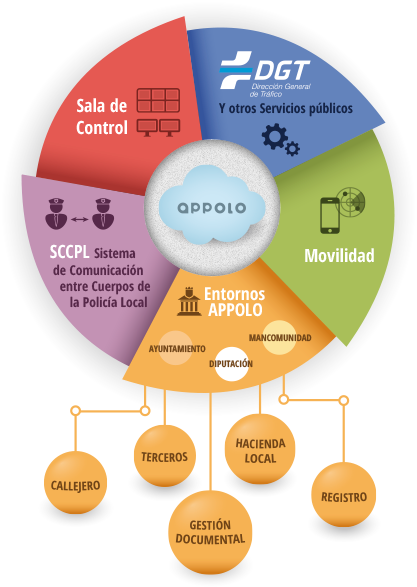
\includegraphics[scale=0.55]{imagenes/appolo-info.png}
	\caption{Bloques que conforman Appolo.\cite{appolo} \label{fig:figura15}}
\end{figure}

Esta aplicación se rige bajo una licencia \textit{open source} pero bajo pago. Por tanto, no podemos conocer el código de la aplicación
sin haber pagado por la licencia. El sistema de cobro que usan es el basado en tarifa plana, por lo cual se deberá pagar en un
único plazo y antes de comenzar a utilizar la aplicación. Esto ocasiona una gran barrera en el momento de querer comenzar a utilizar esta aplicación ya que hasta que no obtenemos la licencia, no podremos saber si se adapta a las necesidades que tenemos o si es realmente útil para los agentes.

\section{Crítica al estado del arte}

Después de analizar las aplicaciones anteriores, se puede concluir que \textbf{no} existe una aplicación
de código libre, gratuita y en la que los desarrolladores de la comunidad puedan involucrarse de manera activa.
Las aplicaciones anteriores no son muy usadas debido a su alto precio. En la mayoría de los casos, las instituciones
no pueden permitirse este gasto y no cambian el modelo que están utilizando actualmente.\\


Con esta aplicación se podrá llegar donde las anteriores aplicaciones no han llegado. De este modo al tener en cuenta un mayor sector de posibles usuarios, 
\textbf{Chief} puede conseguir una mayor implantación en el mercado. Esto puede provocar que la comunidad de desarrolladores vea una buena oportunidad y se involucre 
de manera activa en el proyecto, consiguiendo mejoras y atendiendo a las necesidades de la comunidad.

\section{Propuesta}

Se propone crear el \textbf{primer} sistema de ayuda a la labor policial de código libre y completamente gratuito que cuente
con el apoyo directo de un órgano del Estado. Este proyecto puede significar una gran paso para la aceptación 
del código libre como una alternativa igual de válida que el código cerrado para un sector en el 
que hasta ahora, no ha tenido cabida.\\  
